\section{Experiments}\label{sec:results}
To successfully perform the NA-task, the LSTM should: (1) encode and store the grammatical number of the subject; and (2) track the main subject-verb syntactic dependency. The latter information is important for identifying the time period during which the network should store the subject number, and when it should output it and allow to update number information. This section describes the `neural circuit' that encodes and processes this information in the LSTM.

\begin{center}
\begin{table}[ht]
\centering
\begin{tabular}{|P{2.3cm}|P{0.4cm}||P{0.6cm}|P{0.6cm}|P{0.6cm}|}
\hline
    \B \multirow{2}{*}{NA task} & \B \multirow{2}{*}{C} & \multicolumn{2}{c|}{\B Ablated}& \multirow{2}{*}{\B Full} \\
    \cline{3-4}
    & & \B \textbf{\unit{2}{126}} & \B \textbf{\unit{2}{338}} & \\
\hline

% Singular conditions
Simple & S & - &  - &  \textcolor{red}{100} \\

Adv & S & - &  - &  \textcolor{red}{100} \\

2Adv & S & - &  - &  \textcolor{red}{99.9} \\

CoAdv & S & - &  \textcolor{red}{82} &  \textcolor{red}{98.7} \\

namePP & SS & - &  - &  \textcolor{red}{99.3} \\

nounPP & SS & - &  - &  \textcolor{red}{99.2} \\

nounPP & SP &  - &  \textcolor{red}{54.2} &  \textcolor{red}{87.2} \\

nounPPAdv & SS &  - &  - & \textcolor{red}{99.5} \\

nounPPAdv & SP &  - &  \textcolor{red}{54.0} & \textcolor{red}{91.2} \\


\hline
% Plural conditions
Simple & P &  - &  - &  \textcolor{blue}{100} \\

Adv & P &  - &  - &  \textcolor{blue}{99.6} \\

2Adv & P & - &  - &   \textcolor{blue}{99.3} \\

CoAdv & P &  \textcolor{blue}{79.2} &  - &   \textcolor{blue}{99.3} \\

namePP & PS & \textcolor{blue}{39.9} &  - &   \textcolor{blue}{68.9} \\

nounPP & PS &  \textcolor{blue}{48.0} & - &   \textcolor{blue}{92.0} \\

nounPP & PP &  \textcolor{blue}{78.3} & - &   \textcolor{blue}{99.0} \\

nounPPAdv & PS & \textcolor{blue}{63.7} &  - &   \textcolor{blue}{99.2} \\

nounPPAdv & PP & - &  - &   \textcolor{blue}{99.8} \\

\hline

\B Linzen & \B - &   75.3 &  - &  93.9 \\
\hline

\end{tabular}
% \tiny
\caption{Ablation-experiments results: Percentage accuracy in all NA-tasks. Full: non-ablated model, C: condition, S: singular, P: plural. Red: Singular subject, Blue: Plural subject. Performance reduction less than 10\% is denoted by `-'.  \label{tab:ablation-results}}
\end{table}
\end{center}

\begin{figure*}[ht]
    \centering
    \begin{subfigure}{\textwidth}
            \centering
            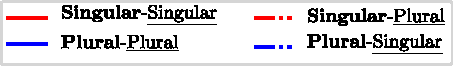
\includegraphics[width=0.3\linewidth]{Figures/legend.pdf}
    \end{subfigure}
    \bigskip
    \begin{subfigure}{0.32\textwidth}
            \centering
            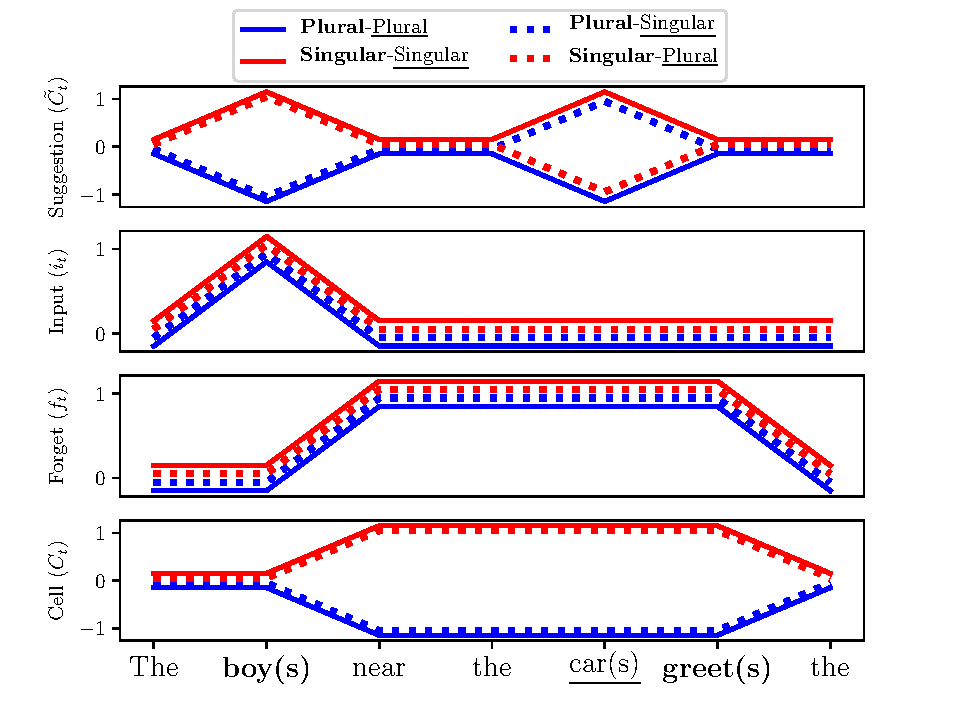
\includegraphics[width=\linewidth]{Figures/unit-timeseries-cartoon.pdf}
            \subcaption{Prediction (singular)}
    \label{fig:cartoon}
    \end{subfigure}
    \begin{subfigure}{0.32\textwidth}
            \centering
            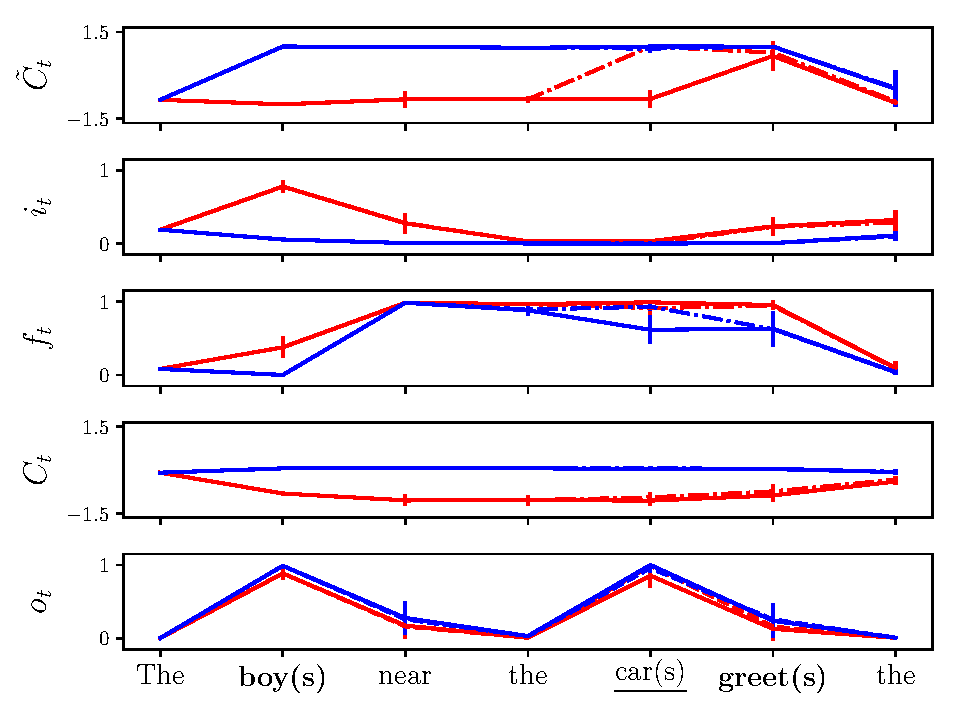
\includegraphics[width=\linewidth]{Figures/nounpp_987.pdf}
            \subcaption{\unit{2}{338} (singular)}
    \label{fig:singular-unit}
    \end{subfigure}
    \begin{subfigure}{0.32\textwidth}
            \centering
            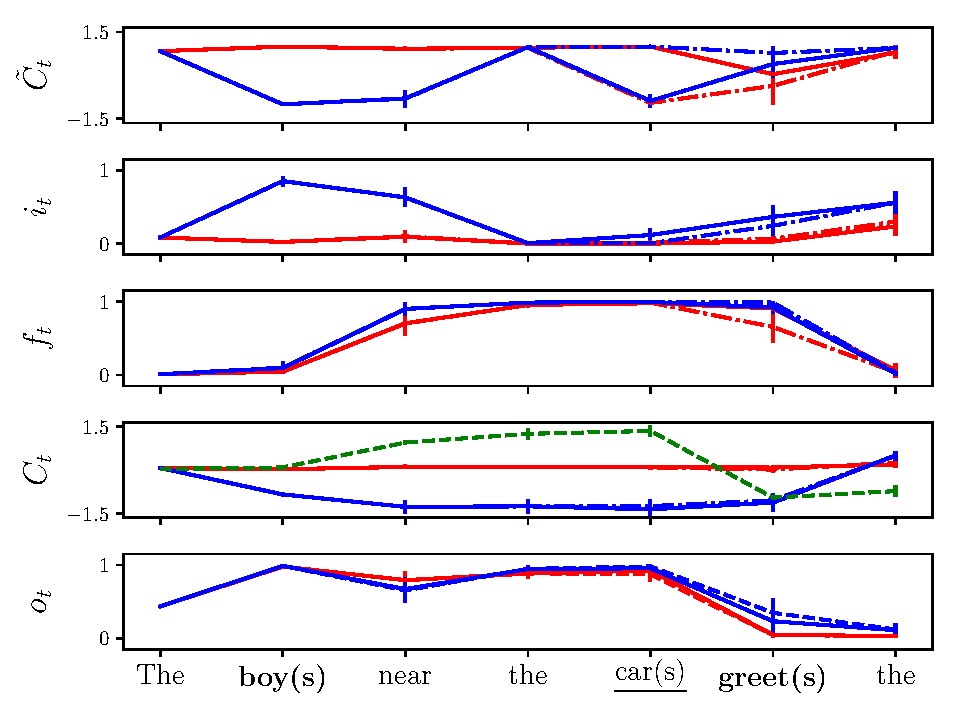
\includegraphics[width=\linewidth]{Figures/nounpp_775.pdf}
            \subcaption{\unit{2}{126} (plural)}
    \label{fig:plural-unit}
    \end{subfigure}
\caption{Cell and gate activations during processing of sentences with a prepositional phrase between subject and verb. Values in (b) and (c) are averaged across all condition sentences, with error bars showing standard deviations.}
\end{figure*}

\subsection{Long-range number units}\label{subsec:ablation}
We first tested LSTM performance on Linzen's data and on the NA-tasks of Table
\ref{tab:data-sets}. Following
\newcite{Linzen:etal:2016} and later work, we computed the likelihood
that the LSTM assigns to the main verb of each sentence given the
preceding context, and compared it to the likelihood it assigns to the
wrong verb inflection. Accuracy in a given condition was measured as the proportion of sentences in the condition where the model assigned a higher likelihood to the correct form than to the wrong one.

Network performance is reported in Table \ref{tab:ablation-results}
(right column -- `Full'). First, results show that some NA-tasks and
conditions are more difficult than others. For example, performance on
the Simple (0-distance) NA-task is better than that on the Co-Adv
NA-task, which in turn is better than that of the nounPP
tasks. Second, as expected, incongruent conditions (the
number-mismatch conditions of namePP, nounPP and nounPPAdv) reduce
network performance. Third, for long-range dependencies, reliably
encoding singular subject across an interfering noun is more difficult
than a plural subject: for both nounPP and nounPPAdv, PS is easier
than SP. A possible explanation for this finding is that in English the plural form is
almost always more frequent than the singular one, as the latter only
marks third person singular, whereas the former is identical to the
infinitive and other forms. Thus, if the network reverts to unigram
probabilities, it will tend to prefer the plural. Last, we replicated
the results of \newcite{Gulordava:etal:2018} for the Linzen NA-task.

\paragraph{Looking for number units through ablation} Number
information may be stored in the network in either a local, sparse, or
a distributed way, depending on the fraction of active units that
carry it.  We hypothesized that if the network uses a local or sparse
coding, meaning that there's a small set of units that encode number
information, then ablating these units would lead to a drastic
decrease in performance in the NA-tasks.  To test this, we ablated
each unit of the network one at a time, by fixing its activation to zero,
and tested on the tasks.

Two units were found to have exceptional effect on network performance
(Table \ref{tab:ablation-results}, \unit{2}{126} and \unit{2}{338}
columns).\footnote{Units 1-650 belong to the first layer, 651-1300 to
  the second. All units detected by our analyses come from the latter.} Ablating them reduced network performance by more than 10\%
across various conditions, and importantly, they were the only units
whose ablation consistently brought network performance to around
chance level in the more difficult incongruent conditions of the
namePP, nounPP and nounPPAdv
tasks. 

Moreover, the ablation effect depended on the grammatical number of the subject: ablating \unit{2}{126} significantly reduces
network performance only if the subject is plural (P, PS or PP conditions) and \unit{2}{338}
only if the subject is singular (S, SP or SS conditions). In what follows, we will therefore
refer to these units as the `plural' and `singular' units, respectively,
or long-range (LR) number units when referring to both. Finally, we note that although the Linzen NA-task contained mixed stimuli from many types of conditions, the plural unit was found to have a substantial effect on average on network performance. The singular unit didn't show a similar effect in this case, which highlights the importance of using carefully crafted stimuli, as in the nounPP and nounPPAdv tasks, for understanding network dynamics. Taken
together, these results suggest a highly local coding scheme of
grammatical number when processing long-range dependencies.

\paragraph{Visualizing gate and cell-state dynamics}\label{subsec:gate-dynamics}
To understand the functioning of the number units, we now look
into their gate and state dynamics during sentence processing. We
focus on the nounPP NA-task, which is the simplest NA-task including a
long-range dependency having an interfering noun in both SP and PS
incongruent conditions.

Recall the standard LSTM memory update and output rules \cite{Hochreiter:Schmidhuber:1997}:
\begin{align} 
    C_t &= f_t\circ C_{t-1} + i_t\circ \widetilde{C}_t \label{eq:update-rule} \\
     h_t &= o_t\circ \tanh(C_t) \label{eq:output},
\end{align}
where $f_t, i_t, o_t \in (0,1)$ are gating scalars computed by the network, and $\widetilde{C}_t \in (-1, 1)$ is an update candidate for cell value.

Consider now how a number unit may reliably encode and store subject
number across interfering nouns.  Figure\ref{fig:cartoon} exemplifies
this for a singular unit, showing the desired gate and cell
dynamics. The four conditions are represented with separated curves -
red for singular subject, blue for plural, and dashed lines for
incongruent conditions. Gate and cell activity at time points
unrelated to solving the NA-task are masked with white, as we do not
make precise predictions for them.

The update rule of the LSTM cell has two terms
(Eq.~\ref{eq:update-rule}).\footnote{We abuse notation here, using the
  symbols denoting whole layers in equations (\ref{eq:update-rule}) and
  (\ref{eq:output}) to denote the components of single cells.} In the
first, $f_t \circ{} C_{t-1}$, the forget gate controls whether to keep
the previous cell content ($f_t=1$: perfect remembering) or forget it
($f_t=0$: complete forgetting). In the second,
$i_t\circ{} \tilde{C}_t$, the input gate controls whether the
information currently presented to the network, as encoded by
$\tilde{C}_t$, should be written onto the cell ($i_t=1$: full access)
or not ($i_t=0$). The singular unit can thus use these gates to
reliably store number information across long-range
dependencies. Specifically, the unit can (enumeration follows the same order as the panels in Figure~\ref{fig:cartoon}): (1) encode subject
number via $\tilde{C}_{t_{subject}}$ with different values for
singular and plural; (2) open the input gate \textit{only} when a
singular subject is presented ($i_{t_{subject}} = 1$ in red curves \textit{only}) and protect it from interfering nouns ($i_t=0, t_{subject}<t<t_{verb}$); (3) at the same time,
clear the cell from previously stored information
($f_{t_{subject}}=0$) and then store subject number across the entire
dependency ($f_t=1, t_{subject}<t<t_{verb}$); (4) this will result in
stable encoding of subject number in the cell $C_t$ throughout the
dependency; (5) finally, output subject number at the right moment,
when predicting the verb form ($o_{t_{verb}-1}=1$)
(Eq.~\ref{eq:output}).

Figures \ref{fig:singular-unit} and \ref{fig:plural-unit} present the actual gate and cell dynamics of the singular and plural units. Both units follow the general solution for reliable number storage described above. Note that for $\tilde{C}_t$ and $i_t$, and as a result also for $C_t$, the plural unit `mirrors' the singular unit with respect to subject number (red curves of PP and PS vs. blue curves of SS and SP). This is in accordance with the results of the ablation experiments, which showed that ablating these units had an effect that depended on the grammatical number of the subject (Table \ref{tab:ablation-results}). This provides complementary support for the identification of these units as `singular' and `plural'.

A single divergence between the solution depicted in Figure \ref{fig:cartoon} and the actual dynamics of the number units is that input gate activity is smaller, but not zero, at the time step immediately following the subject. One speculative explanation is that this might be useful to process compound nouns. In these cases, subject number information is stored with the second noun, whereas in the case of simple nouns there is no `risk' of encountering an interfering noun immediately after the subject, making the delay in closing the gate safe.

\begin{figure}[b]
    \centering
    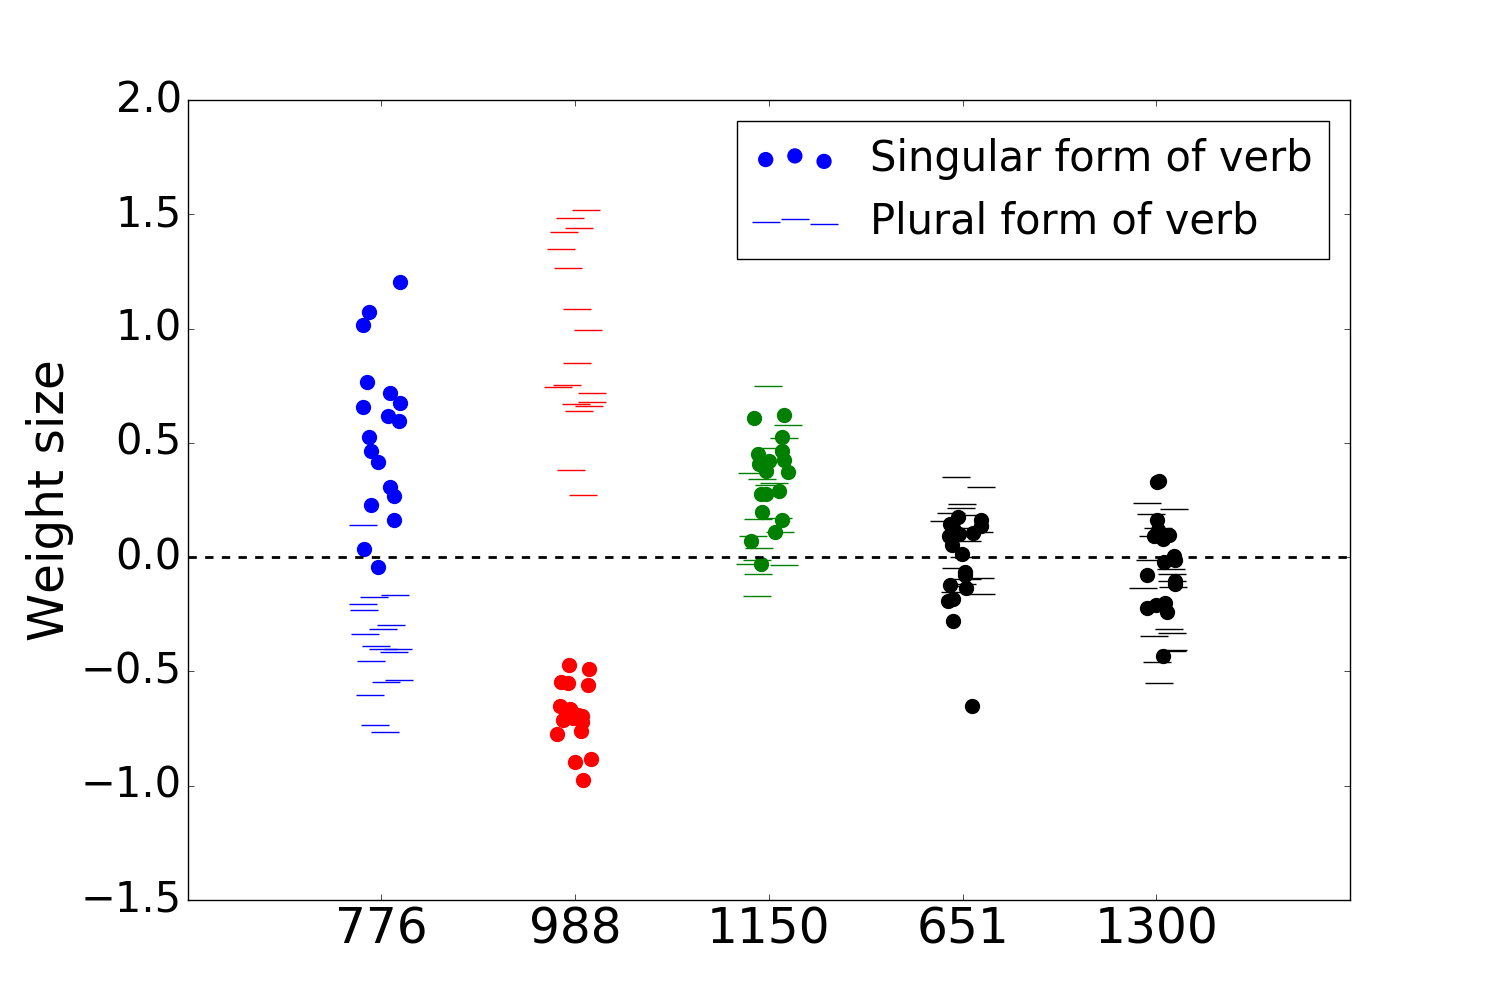
\includegraphics[height=4.6cm]{Figures/weight_dists_verbs.png}
    \caption{Efferent weights of the LR-units (\unit{2}{126} and \unit{2}{338}), the syntax unit (\unit{2}{500}; section \ref{sec:syntax-units}) and two arbitrary units (\unit{2}{1} and \unit{2}{650}).}
    \label{fig:output-weights}
\end{figure}

The singular and plural units had emerged at the second layer of the network. This seems appropriate if number information needs to be directly projected to the output layer for correct verb-form prediction. Moreover, number-unit output should be projected differently to singular and plural verb forms in the output layer, only increasing activity in output units representing the suitable form. For example, for the singular unit, since singular subjects are encoded with a negative value ($C_{t_{verb}-1}<-1$ in figure \ref{fig:singular-unit}), the more negative its efferent weights to singular verb forms in the output layer, the higher the probabilities of these verb forms would be. Figure \ref{fig:output-weights} shows the efferent weights of the LR-number units to all verbs in our data-sets. We found that, indeed, the efferent weights to the singular and plural verb forms are segregated from each other, with weight signs that correspond to the negative encoding of subject number used by both singular and plural units. Two other arbitrary units, \unit{2}{1} and \unit{2}{650}, and the syntax unit \unit{2}{500} to be described below (Section \ref{sec:syntax-units}) do not have segregated efferent weights to verb forms, as expected. 

\subsection{Short-range number information}
\begin{figure}
    \centering
    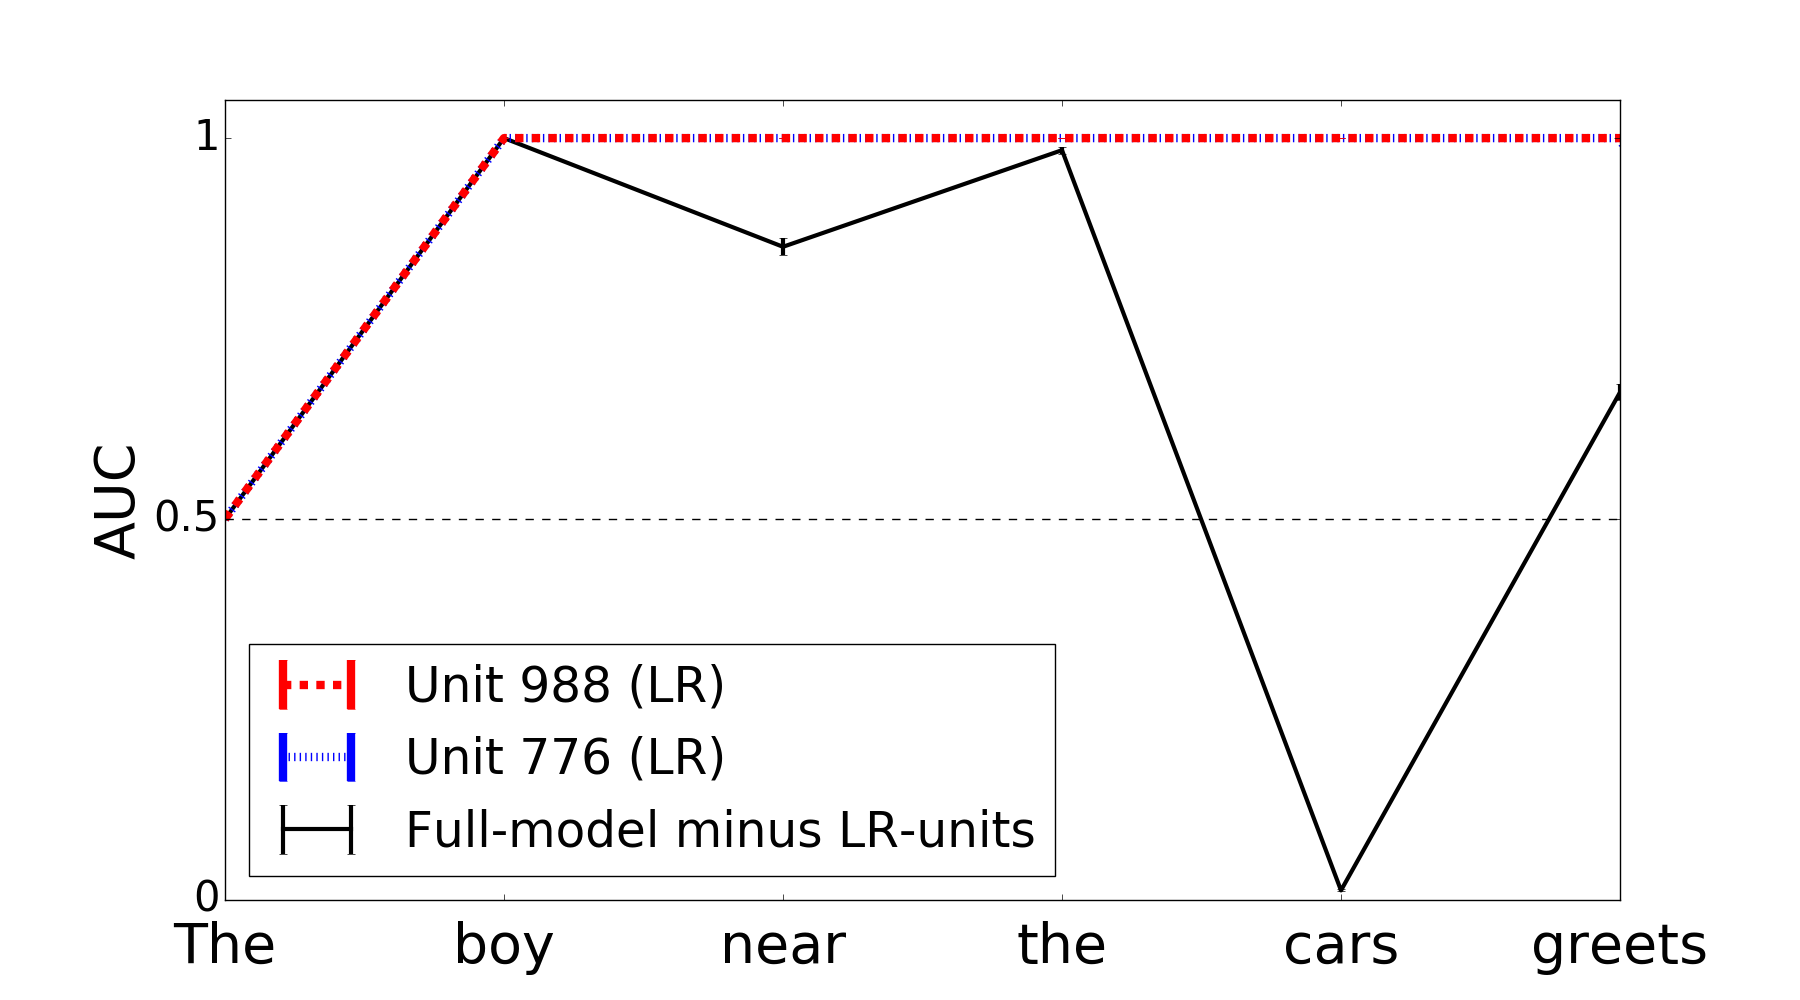
\includegraphics[height=4cm, width=8cm]{Figures/GAT1d_cell_.png}
    \caption{Generalization across time of subject-number prediction. Error bars represent standard deviations across cross-validation splits.}
    \label{fig:GAT}
\end{figure}

Performance on the easier NA-tasks (Simple, Adv, 2Adv) was not
impaired by single-unit ablations. This suggests that number may be
encoded also elsewhere in the network, perhaps via a more distributed
code. To verify this, we tested whether subject number can be decoded from the whole
pattern of activities in the network (excluding the two LR-number units)
and whether this decoding is stable across time \cite[see][for similar
observations and related methods]{Giulianelli:etal:2018}. We expected
this distributed activity network to track number in a
small time window after the subject, but, unlike the LR-number units,
to be affected by incongruent intervening nouns.

We trained a linear model to predict the grammatical number of the
subject from network activity in response to the presentation of the
subject, and tested its prediction on test sets from all time points
\cite{King:Dehaene:2014}, in incongruent conditions only of the nounPP
task. We used Area under of Curve (AUC) to evaluate model
performance. Figure \ref{fig:GAT} shows decoding across time of
subject number from cell activity of each number unit separately and
from cell activity of the entire network without these two units
(`Full model minus LR-units'). Results show that number information
can be efficiently decoded from other units in the network, and that
this information can be carried for several time steps (relatively
high AUC up to the second determiner). However, the way in which these
units encode number is sensitive to the last encountered noun, with
AUC decreasing to zero around the second noun (`cars'), whereas test
performance of the models trained on cell activity of the LR-number
units is consistently high. This confirms that number prediction is
supported both by the LR-number units, and by distributed activation
patterns of other short-range (SR) number units. The latter, however,
are not syntax-sensitive, and simply encode the number of the last
noun encountered.

%A full description of the SR-number units is beyond our scope. We
%tried however to identify specific SR-number units by training a
%linear model to predict subject number from single-unit activations,
%and by a careful inspection of the weights of a classifier trained on
%the full model (Figure \ref{fig:GAT}), accompanied by informal
%inspection of unit dynamics.

A full description of the SR-number units is beyond our scope. However, we note that 10 SR-number units in the second layer of the
network were identified, which had efferent weights with a similar segregated
structure as that of the LR units (Figure
\ref{fig:output-weights}). These units were indeed sensitive to the last
encountered noun: subject number could be decoded from single-unit cell activity
during its presentation (AUC$>0.9$), but activity `swaps' once an
interfering noun appears (i.e., AUC decreases to zero in a
generalization-across-time analysis). Finally, to validate the role of SR-number units in encoding number for easier NA-tasks, we ablated both SR and LR number
units (12 in total) or SR units only (10 in total) and evaluated network performance on these NA-tasks. Both experiments resulted in a significant reduction in task performance compared to 1,000 random equi-size ablations ($p<0.01$ in all `easier' tasks).

Intriguingly, we observed qualitatively that LR units are almost
always making the right prediction, even when the network predicts the
wrong number. The wrong outcome, in such cases, might be due to
interference from the syntax-insensitive SR units. We leave the study of LR-SR
unit interplay to future work.

